\documentclass{article}
\usepackage{nips12submit_e,times}

\usepackage{amsmath}
\usepackage{amsfonts}
\usepackage{amssymb}
\usepackage{graphicx, subfigure, fink, grffile, placeins}
\usepackage{hyperref}
\usepackage{color}
\usepackage{url}
\usepackage{algorithm}
\usepackage{algpseudocode}
\usepackage{upgreek}

% \title{Modeling Network and Text Structure in Online Forums}
% \title{Simultaneous text \& Network modeling in MMSB for Learning Structured
% Interactions on Online Forums}
% \title{Modeling Structured Interaction in Big Online User Forums }
\title{Modeling Structured Interaction in \\ Large Online User Forums }

% \author{
% Abhimanu Kumar \\
% Carnegie Mellon University\\
% \texttt{abhimank@cs.cmu.edu}\\
% \And
% Chong Wang \\
% Carnegie Mellon University\\
% \texttt{chongw@cs.cmu.edu}\\
% \And
% Carolyn P. Rose \\
% Carnegie Mellon University\\
% \texttt{cprose@cs.cmu.edu}\\
% }

\newcommand{\fix}{\marginpar{FIX}}
\newcommand{\new}{\marginpar{NEW}}
\newcommand{\comment}[1]{{\color{red}{#1}}}

%\nipsfinalcopy

\begin{document}
\maketitle
\begin{abstract}
We present here an approach to model online social forums that respects the
structure of the discussion and thus inturn provides researchers with unique
insights into the myriads of user forums in the todays online world. We
bring together the structure of the forum as well as texts posted there
in a model that respects the structure of the conversation in the forum. The
model incorporates the strength of interaction among user as well, as compared
to binary case that cares just for presence or absence of interaction. The
work has a scalability focus and provides an efficient approximate estimation 
technique based off stochastic variational methods and is scalable to very
large forums.
%~(\comment{I am thinking of using stochastic variational for
%scalability if time permits.}).
Analysing Wikipidia edits and cancer patients online user forums using this 
technique provides us interesting insights into these communities.
We also perform a set of prediction tasks to validate our claim
further.
%~(\comment{We need to decide this soon, though it hinges on once the
% final model is coded and we have analysed the data using it})
\end{abstract}

\section{Introduction}
Online forums are a microcosm of communities where users' presentation
characteristics vary across different parts of the forum. Users participate in a
discussion or group activity by posting on a related thread. And during his
stay in a forum, a user participates in many different discussions and posts on multiple
threads. The thread level presentation characteristics of a user are different
than the global presentation chracteristics. A participating user gears his
responses to suit specific discussions on different threads. These thread based
interactions give rise to active sub-networks, within the global network of users,
that characterize the dynamics of interaction. Overlaying differential changes
in user interaction characteristics across these sub-networks provides
insights into users' macroscopic (forum-wide) as well as microscopic (thread
specific) participation behavior. 

Analysing online social networks and user forums have been approached using
various perspective such as graph/network ~\cite{Shi:2000:NCI:351581.351611,
Shi00learningsegmentation} , probabilistic 
graphical model~\cite{ Airoldi:2008:MMS:1390681.1442798}, 
combined network \& text mining
based~\cite{Ho:2012:DHT:2187836.2187936,Nallapati:2008:JLT:1401890.1401957}
based approaches. But none of the approches above in social networks have taken
into account the dynamics of sub-networks and the related thread-based structural framework in
which the discussions in online forums happen. Whereas active-subnetwrok modelling has
been very useful to the research in computational biology in recent years where
it's been used to model sub-network of gene
interactions~\cite{journals/ploscb/DeshpandeSVHM10,Lichtenstein:Charleston},
very few approaches using active-subnetwork have been proposed to model online
forum user interactions. Taking into account subnetwork interaction
dynamics is important to correctly model the user particiaption behavior. E.g.
in an onlne forum there are topic-threads and users post their responses on
these threads after possibly reading through the responses of other users in
these threads. The users possibly post multiple times on the thread in the form
of replies to other posts in the thread. For analysing such a user interaction it
becomes imperative that the structure of the conversation must also be taken
into account  besides taking into account the user interaction network and the
text posted. This enables us to gain deeper insights into user behavior in the
online community that was not possible earlier. 

One of the main challenges of this work has been the ability to deal with
social network data on a large (millions of users and threads) scale. A
social network spanning around millions of users and threads would be an ideal
case to demonstrate effectiveness of active-subnetwprk modelling. To this
purpose we designed a model based on Stochastic variational 

The model also incorporates strength of interaction
among the users by incorporating interaction counts as compared to MMSB model
which just looks presence or absence of link~\cite{Airoldi:2008:MMS:1390681.1442798}. 
In the process we discover interesting online communities and social phenomena.

The current work also focuses on analysing large scale user interactions in big
online social forums. We provide a stochastic variational
approximation~\cite{Hoffman:2013:SVI} based estimation technique that is
scalable to big forums with thousands of users.

% ~\comment{Also write about stochastic approximation if given we have time and we
% can get it working}. 



\section{Related Work}
Our project lies at the intersection of community discovery, structure modelling
and text mining. Wikipedia's talk pages are an instance of a large social
community where we can observe users networking with each other as well as
posting content in a structured way. Similar phenomena are observed across
almost all social networking websites and online forums.


For role-identification and clustering users based on roles in online communities, 
White et al.\cite{ICWSM124638} proposed a mixed-membership model that obtained
membership probabilities for discussion-forum users for each statistic
(in- and out-degrees, initiation rate and reciprocity) in various profiles and 
clustered the users into ``extreme profiles''. In a similar work, Ho et al.
\cite{Ho:2012:DHT:2187836.2187936} presented TopicBlock that combines text and 
network data for building a taxonomy for a corpus. 
The LDA model and MMSB models were combined by
Nallapati et al. \cite{Nallapati:2008:JLT:1401890.1401957} using the
Pairwise-Link-LDA and Link-PLSA-LDA models where documents are assigned
membership probabilities into bins obtained by topic-models.

For simultaneously modeling topics in bilingual-corpora, Smet et al.
\cite{Smet:2011:KTA:2017863.2017915} proposed the Bi-LDA model that generates
topics from the target languages for paired documents in these very languages.
The end-goal of their approach is to classify any document into one of the
obtained set of topics. For modeling the behavioral aspects of entities and
discovering communities in social networks, several game-theoretic approaches
have been proposed (Chen et al. \cite{Chen:2010:GFI:1842547.1842566}, Yadati and
Narayanam \cite{Yadati:2011:GTM:1963192.1963316}). Zhu et
al.~\cite{Zhu:getoor:MMSB-text} combine MMSB and text for link prediction and
scal it to 44K links.

Ho et al.~\cite{HoYX12} provide a unique triangulated sampling schemes for scaling
mixed membership stochastic block models~\cite{Airoldi:2008:MMS:1390681.1442798} to
hundreds of thousands users based communities. Prem et al.~\cite{conf/nips/GopalanMGFB12}
use stochastic variational inference coupled with sub-sampling techniques to
scale MMSB like models to hundreds of thousands of users.

None of the works above address the strucutre of the information flow in an
online community. Our work is unique in this context as it tries to bridge the
gap between community discovery and strucured interaction. We propose a novel
modelling scheme that takes into account the network information, user contents
as well as structure of the interaction and is scalable to big online forums.


% \section{Graphical Model \& Generative Story}
\section{Approach}
\label{sec:approach}
Online forums generally have a specific structure that provides a lot of
context to all the interactions occuring among the users. Ignoring this in the
analysis makes researhers lose a lot of precious information as we will see in
later sections.
Here we describe a typeical forum \& related structure and the answers that we
are looking for.

\subsection{Structure in online forums}
In an online forum when two users interact in a thread or through a post
they probably bring from their own individual point of views or come
form possibly different communities.
It is valuable to know which topic/community they each belong to in that
interaction. When a user U is representing community C out of all communties
that he is part of, he tailors his post content accordingly to suit the
explicit or implicit community norms. Knowing the style of community
specific text content provides a lot of information about the community in general. 
It also provides information about what role user U plays when he is in community
C. In online forums multi-user interactions happen a lot i.e.
in a thread a user can post by addressing to another specific user but he is
also addressing other users in the thread explicitly or implicitly. Modeling
this phenomenon would bring our model closer to reality. This knowledge 
can be modelled by aggregating
users posts acorss a thread, though not across the whole of the forum. We will
elaborate on this more in the generative story section.
Another interesting property of such structured conversations is that there is 
an inherent bias towards the thread starter or in turn topic of the thread. 
It would be interesting to see what 
insights this knowledge provides given that a model can make use of such an
information (\comment{This would be very relevant for post-and-response
forums in our dataset such as Reddit and Stack Overflow. Right now our graphical
model doesn't support this but it would be interesting to see how this can be brought in. It might not be too difficult to do this}).


\subsection{Graphical model \& generative story}
Based on the discussions above our graphical model is designed as shown
in figure~\ref{fig:finalThreadAggregationModel}. In this model,
figure~\ref{fig:finalThreadAggregationModel} below, we aggregate the posts of 
a given user in a given thread into one document called $R_p$. This helps us
incorporate the knowledge that a user's post is influenced by all the posts of
other users present on the thread.

The generative process for the model is as follows:

\begin{figure}
\centering
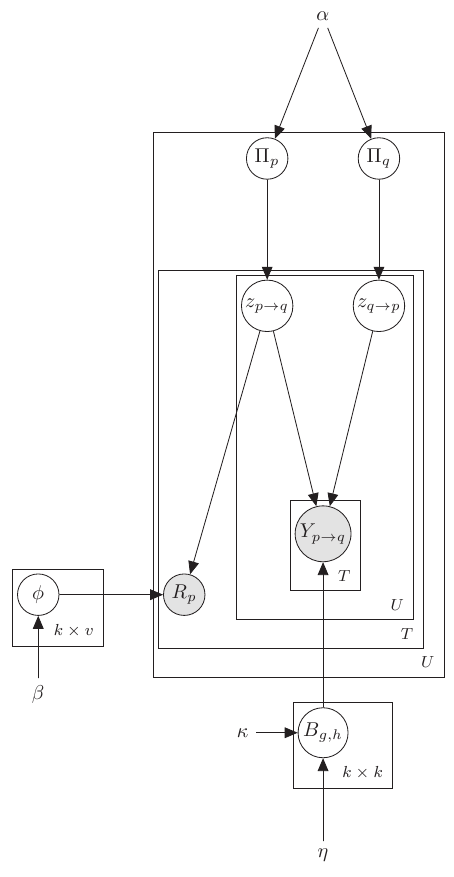
\includegraphics[width=0.6\textwidth]{pgm_ThreadBased.png}
\caption{This graphical model takes into account multi-way interaction among
users in a thread simultaneously}
\label{fig:finalThreadAggregationModel}
\end{figure}

Assuming that there are total $N_t$ users in the thread $t$.  
\begin{itemize}
  \item For each Thread $t$
\begin{itemize}
  \item For each user $p \in \mathcal{N}_t$
  \begin{itemize}
    \item Draw a $K$ dimensional mixed membership vector 
    $\overset{\rightarrow}{\uppi}_{p} \sim$ Dirichlet($\alpha$)

    \item Draw $B(g,h) \sim Gamma(\kappa,\eta)$; where $\kappa, \eta$ are
    parameters of the gamma distribution.
  \end{itemize}

  \item For each pair of users $(p, q) \in \mathcal{N}_t \times \mathcal{N}_t$:
  \begin{itemize}
    \item Draw membership indicator for the indicator, 
    $\overset{\rightarrow}{z}_{(p \rightarrow q,t)} \sim$
    Multinomial($\uppi_{p}$).
    \item Draw membership indicator for the receiver,
    $\overset{\rightarrow}{z}_{(q \rightarrow p,t)} \sim$
    Multinomial($\uppi_{q}$).
    \item Sample the value of their interaction, $Y(p,q,t) \sim$
    Poisson(${\overset{\rightarrow}{z}}^{\top}_{(p \rightarrow q,t)}
    B~\overset{\rightarrow}{z}_{(p \leftarrow q,t)}$). 
	\end{itemize}
	\item For each user $p \in \mathcal{N}_t$
	\begin{itemize}
	  \item Draw $\phi_{k}$ from $Dirichlet(\beta)$.
	  \item Form the set $Q_{p,t}$ that contains all the users that p interacts to
	  on thread $t$
	  \begin{itemize}
	    \item For each word $w \in R_{p,t}$ 
	    \item Draw $w \sim \phi(w|z_{(p \rightarrow q,t)}, \forall q\in Q_{p,t})$  
	  \end{itemize}
  \end{itemize}
\end{itemize}  
\end{itemize}

The data likelihood for the model in figure~1

\begin{eqnarray}
P(Y, R_{p} | \alpha, \beta, \kappa, \eta) = \int_{\Phi} \! \int_{\Pi} \sum_{z} \! P(Y, R_{p}, z_{p \rightarrow q}, z_{p \leftarrow q}, \Phi, \Pi | 
\alpha, \beta, \kappa, \eta)  \nonumber \\  \nonumber
\\ = \int_{\Phi} \! \int_{\Pi} \sum_{z} \! \bigg[ \prod_{p,q} \prod_{t}
P(Y_{pq}^{t} | z_{p \rightarrow q}^{t}, z_{p \leftarrow q}^{t}, B) 
\cdot P(z_{p \rightarrow q}^{t} | \Pi_{p}) \cdot P(z_{p \leftarrow q}^{t} |
\Pi_{q})  \nonumber
\\ \cdot \left(\prod_{p} P(\Pi_{p} | \alpha) \prod_{t} \prod_{p} P(R_{p}^{t} |
z_{p \rightarrow q}^{t}, \Phi) \cdot \prod_{k} P(\Phi_{k} | \beta)\right) \cdot
\prod_{g,h}P(B_{gh} | \eta, \kappa) \bigg]
\end{eqnarray}

The complete log likeliood of the model is:

\begin{align}
\log \! P(Y, W, z_{\rightarrow}, z_{\leftarrow}, \Phi, \Pi, B | \kappa, \eta,
\beta, \alpha) = \sum_{t} \! \sum_{p,q} \! \log P(Y_{pq}^{t} | z_{p \rightarrow
q}^{t} , z_{p \leftarrow q}^{t}, B)~+ \nonumber  \\\nonumber \sum_{t} \!
\sum_{p,q} \! (\log P(z_{p \rightarrow q}^{t} | \Pi_{p}) + \log \! P(z_{p \leftarrow q}^{t} |
\Pi_{p})) + \sum_{p} \! \log \! P(\Pi_{p} | \alpha) ~+\\  \sum_{t} \!
\sum_{p} \! \sum_{w \in R_{p}^{t}} \log P(w | z_{p \rightarrow}, \Phi) +
\sum_{k} \! \log P(\Phi_{k} | \beta) + \sum_{gh} \! \log P(B_{gh} | \eta,
\kappa)
\end{align}

The mean field variational approximation for the posterior is 

\begin{align}
q(z, \Phi, \Pi, B | \Delta_{z_{\rightarrow}}, \Delta_{\Phi}, \Delta_{B},
\Delta_{z_{\leftarrow}}, \Delta_{B_{\kappa}}) = \prod_{t} \! \prod_{p,q} \!
\bigg( q_{1}(z_{p \rightarrow q}^{t} | \Delta_{z_{p \rightarrow q}}) +
q_{1}(z_{p \leftarrow q}^{t} | \Delta_{z_{p \leftarrow q}})  \bigg) \nonumber \\
\cdot \prod_{p} \! q_{4}(\Pi_{p} | \Delta_{\Pi_{p}}) \prod_{k} q_{3} (\Phi_{k} |
\Delta_{\Phi_{k}}) \prod_{g,h} \! q(B_{g,h} | \Delta_{B_{\eta}}, \Delta_{B_{\kappa}})
\end{align}

The lower bound for the data log-likelihood from jensen's inequality is: 

\begin{align}
L_{\Delta} &= E_{q}\bigg[ \log \! P(Y, W, z_{\rightarrow}, z_{\leftarrow}, \Phi,
\Pi, B | \kappa, \eta, \beta, \alpha) - \log \! q \bigg]
\end{align}

\begin{eqnarray}
L_{\Delta} = E_{q} \Bigg[ \sum_{t} \! \sum_{p,q} \! \log \left(
B_{g,h}^{Y_{p,q}^t} \frac{e^{-B_{gh}}}{Y_{pq}^{t}!} \right) +
\sum_{t} \! \sum_{pq} \! \log\left( \prod_{k} (\pi_{p,k}^{z_{p \rightarrow q} =
k}) \right) + \sum_{t} \! \sum_{p,q} \log \! \left( \prod_{k}(\pi_{q,k})^{z_{p
\leftarrow q} = k} \right) ~+ \nonumber\\
 \sum_{p} \! \log \left( \prod_{k}
(\Pi_{p,k})^{\alpha_{k} - 1} \cdot \frac{\Gamma(\sum \alpha_{k})}{\prod_{k}
\Gamma(\alpha_{k})} \right) +
\sum_{t} \! \sum_{p} \! \sum_{w\in R_p^t}  \log \! \left(
\prod_{u\in V}(\bar{z}^T\phi_u)^{w = u} \right) + \nonumber\\
 \sum_{k} \! \log\left( \prod_{u\in V}
(\phi_{k,u})^{\beta_{k} - 1} \cdot \frac{\Gamma(\sum \beta_{k})}{\prod_{k}
\Gamma(\beta_{k})} \right) +
 \sum_{g,h} \! \log \! \left( B_{g,h}^{\kappa - 1} /
\eta^{\kappa} \Gamma(\kappa) \cdot \exp(-B_{g,h}/\eta) \right) \Bigg]
\nonumber\\
% 
% \end{eqnarray}
% \begin{eqnarray}
 -E_{q} \Bigg[ \sum_{t} \! \sum_{p,q} \log \big( \prod_{k} (\Delta_{z_{p
\rightarrow q}, k})^{z_{p \rightarrow q}=k} \big) + \sum_{t} \! \sum_{p,q}
\! \log \! \left(
\prod_{k} \! (\Delta_{z_{p \leftarrow q}, k})^{z_{p \leftarrow q} = k} \right)
 + \nonumber \\
 \sum \! \log \left( \prod_{k} \! (\Pi_{p,k})^{\Delta_{\pi_{pk}}-1}
\frac{\Gamma(\Delta_{\Pi_{p}})}{\prod_{k=1} \! \Gamma(\Delta_{\Pi_{p,k}})}
\right) + 
\sum_{k} \log \! \left( \prod_{u \in v}
(\Phi_{k,u})^{\Delta_{\Phi_{ku}} - 1)} \frac{\Gamma(\Delta_{\Phi_{k}})}
{\prod_{u \in v} \! \Gamma(\Delta_{\Phi_{k,u}})} \right) + \nonumber \\ 
\sum_{g,h} \log \! \left(
\frac{B_{g,h}^{\Delta_{\kappa = 1}}}{\Delta_{\eta}^{\Delta_{\kappa}}
\Gamma(\Delta_{\kappa})} \exp(-B_{g,h}/\Delta_{\eta}) \right) \Bigg]
\label{eqn:VarLowerBound}
\end{eqnarray}


Equation~\ref{eqn:VarLowerBound} is the variational lower bound of the log
likelihood function which is to be maximized.
There are terms like $ E_q\left[\sum_{g,h} \! \log \! \left( B_{g,h}^{\kappa -
1} / \eta^{\kappa} \Gamma(\kappa) \cdot \exp(-B_{g,h}/\eta) \right) \right]$
which can be obtained by taking derivation of the partition function of the exponential
family form of gamma distribution. An effective way
to evaluate $E_q\left[ \sum_{t} \! \sum_{p} \! \sum_{w\in R_p^t}  \log \! \left(
\prod_{u\in V}(\bar{z}^T\phi_u)^{w = u} \right)\right]$ 
is by introducing an additional latent variable $\bar{z}_p$ which is a
realization of the average $\frac{\sum_{q\in Q} z_{p\rightarrow q}}{|Q|}$. 
~\comment{So figure~\ref{fig:finalThreadAggregationModel} will be modifed
slightly in future where $R_p$ is drawn from $\bar{z}$ and $\bar{Z}$ is drawn from
$z_{p\rightarrow q}$. This was suggested by Chong as well as Eric but I
finally figured out the equation of the vriational approximation for this. I
will update the equations once I have coded it and verified.}.


\section{Datasets}











% 
% \section{Our Method \& Tasks Finished}
% Our approach is to model social emergence via designing a mixed membership
stochastic block model when we have a tensor graph of user-user interaction 
instead of just a single user$\times$user matrix as is the case for the
MMSB~\cite{Airoldi:2008:MMS:1390681.1442798}. We define a tensor 
of user$\times$user$\times$interactions tensor $Y_{N,N,I}$, where $N$ is 
the number of users and $I$ is the number of interaction types. The tensor 
$Y$ is the data observed.

\paragraph{Tasks finished.} We have designed a model that can handle a multitude
of interaction types in a network. The model also takes into account non-binary 
edge-weights in the graph. Our present model is a mixed membership
stochastic model with tensor interactions. The individual interaction between the 
users are drawn form a Poisson distribution.
% We have plans to extend this model to
% take into account the text that users write while interacting with each other.
The generative story of the present model is:  
\begin{itemize}
  \item For each user $p \in \mathcal{N}$
  \begin{itemize}
    \item Draw a $K$ dimensional mixed membership vector 
    $\overset{\rightarrow}{\uppi}_{p} \sim$ Dirichlet($\alpha$)

    \item Draw $B_t(g,h) \sim Gamma(\kappa,\eta)$
  \end{itemize}

  \item For each pair of users $(p, q) \in \mathcal{N} \times \mathcal{N}$:
  \begin{itemize}
    \item Draw membership indicator for the indicator, 
    $\overset{\rightarrow}{z}_{p \rightarrow q} \sim$ Multinomial($\uppi_{p}$).
    \item Draw membership indicator for the receiver, $\overset{\rightarrow}{z}_{q
    \rightarrow p} \sim$ Multinomial($\uppi_{q}$).
    \item Sample the value of their $i-th$ interaction, $Y(p,q,i) \sim$
    Poisson(${\overset{\rightarrow}{z}}^{\top}_{p \rightarrow q}
    B_{i}\overset{\rightarrow}{z}_{p \leftarrow q}$). We make the assumption that
    two interactions are independent of each other i.e $Y(p,q,i)$ and $Y(p,q,j)$
    are independent of each other where $i\neq j$.
    \item Draw $z_{u,m}$ topic for user $U$'s document from $\pi_u$.
    \item Draw $\tau_{k}$ from $Dirichlet(\beta)$.
    \item Draw a word $w_{u,m}$ from $\tau_{z}$
  \end{itemize}
\end{itemize}  

The graphical model for this gnerative scheme is shown in figure 1.

\begin{figure}
\begin{center}
\includegraphics[width= 0.3\textwidth]{non_lda}
\label{fig:gmodel}
\caption{This graphical model shows the generative scheme of our approach. T is the number of interaction types}
\end{center}
\end{figure}



\paragraph{Intuition behind the approach.} The model rests its case on the intuition that multiple context of 
interaction with the ability to model non-binary edge weights (which in the case of wikipedia are counts thus 
using Poisson) should provide better cluster. We are able to leverage multiple dimesions of the data and the 
chances of getting finer clusters are much more here. 

The joint likelihood of this model is:
\begin{equation}
p(Y, \overset{\rightarrow}{\uppi}_{1:N}, Z_{\rightarrow},
Z_{\leftarrow}|\overset{\leftarrow}{\upalpha}, B) =
\prod_{p,q}(\prod_{i}{P(Y(p,q,i)|\overset{\rightarrow}{z}_{p \rightarrow q},
\overset{\rightarrow}{z}_{p \leftarrow q}, B_{i}))P(\overset{\rightarrow} {z}_{p
\rightarrow q}|\overset{\rightarrow}{\uppi}_{p})\prod_{p}
{P(\overset{\rightarrow}{\uppi}_{p}|\overset{\rightarrow}{\upalpha})}}
\end{equation}  
where $B$ is the block tensor and $B_i$ represent the block matrix for $i-th$
interaction. The marginal data likelihood for this model is:

\begin{eqnarray}
&&p(Y|\overset{\rightarrow}{\upalpha}, B) = \nonumber\\
&&\int_{\Pi}{\sum_{Z}{\bigg( \prod_{p,q}(\prod_{i}{P(Y(p,q,i)|
\overset{\rightarrow}{z}_{p \rightarrow q}, 
\overset{\rightarrow}{z}_{p \leftarrow q}, B_i)) P(\overset{\rightarrow}{z}_{p
\rightarrow q} | \overset{\rightarrow}{\uppi}_{q}) P(\overset{\rightarrow}{z}_{p
\leftarrow q}|\overset{\rightarrow}{\uppi}_{q})\prod_{p}{P(\overset{
\rightarrow}{\uppi}_{p}|\overset{\rightarrow}{\upalpha})}} \bigg)
d\overset{\rightarrow}{\uppi}}} \nonumber\\
\end{eqnarray} 

For results presented here we use collapsed Gibbs sampling for parameter estimation, though 
we also derived variational updates for our model described in \ref{sec:app-1}.
In this section we report the sampling updates steps. We collapse latent variables 
$\overset{\rightarrow}{z}_{p \rightarrow q}$ and $\overset{\rightarrow}{z}_{p \leftarrow q}$ 
together. 
For Poisson case we have:
 \begin{eqnarray}
    p(z|\alpha) &= \int \! p(z|\phi) \cdot p(\phi|\alpha) \, \mathrm{d}\phi\\ \nonumber
    &= \prod_{p} \int \! {\prod_{q}{\prod_{i}^{k}{\pi_{p,i}^{z_{p \rightarrow q},i}}}  \frac{\prod_{i}^{k}{\pi_{p,i}^{\alpha_{i}}}}{Dir(\alpha_{i})} } \, \mathrm{d} \pi_{p}\\ \nonumber
    &= \prod_{p} \frac{\int \! {\prod_{i}^{k}{\pi_{p,i}^{n_{p_{i}} \rightarrow \alpha_{i}}}} \, \mathrm{d} \pi_{p}}{Dir(\alpha+{i})}\\ \nonumber
    &= \bigg[ \frac{Dir(n_{p}^{i} + \alpha_{i}, \dots)}{Dir(\alpha_{i})} \bigg]
  \end{eqnarray}

where $n_{p}^{i}$ is the number of times user $p$ is assigned cluster $i$. And 

\begin{eqnarray}
    P(Y|\eta, z, \kappa) = \prod_{t=1}^{T} \! \prod_{g,h} \left[ \frac{\Gamma(\sum_{p \in g, q \in h} Y_t(p,q) + \kappa) \cdot (n_{t,g,h} + \frac{1}{\eta})^{-(\sum_{p \in g, q \in h} Y_{t}(p,q) + \kappa)}}{\prod_{p \in g, q \in h} Y_t(p,q)! \cdot \eta^{\kappa} \Gamma(\kappa)} \right]\\ \nonumber
  \end{eqnarray}

where $n_{t,g,h}$ is the number of times cluster pair $g,h$ is picked in the interaction context $t$.
Using the above 2 equations the sampling updates are:
\begin{eqnarray}
    & &p(z_{p \rightarrow q = g}, z_{q \rightarrow p = h} | z_{\neg (p \rightarrow q, p \leftarrow q)}, Y, \eta, \alpha, \kappa)
    =\\ \nonumber & &\prod_{t=1}^{T} \left[  \frac{\prod_{i=1}^{Y_t(p \rightarrow q=g,p \leftarrow q=h)} \! (\sum_{a\in g, b \in h} Y_t(a,b) + \kappa - i)}{Y_t(p,q)} \right] \cdot\\ \nonumber
    & & \prod_{t=1}^{T}\left[\frac{(n_{t,g,h} + \frac{1}{\eta})^{-[\sum_{p \in g, q \in h} Y_{t} (p,q) + k]}}{\left[ \left(n_{t,g,h} + \frac{1}{\eta}^{-(\sum_{p \in g, q \in h} Y_{t}(p,q) + \kappa)} \right) \right]_{\neg (p \rightarrow \leftarrow q)}} \right]  \cdot \\ \nonumber
 & & \frac{(n_p^g + \alpha_g)^{\neg (p \rightarrow q = g)}}{(n_p + \alpha)^{(\neg p \rightarrow q =g)}} \frac{(n_q^h + \alpha)^{\neg (p \leftarrow q = h)}}{(n_q + \alpha)^{(\neg p \leftarrow q =h)}}
\end{eqnarray}

The parameter estimation of $\Pi$ and $B$ is:
\begin{eqnarray}
p(B_t(g,h) | \overset{\rightarrow}{z}, \eta, \overset{\rightarrow}{Y_t}) &= (\sum_{p \in g, q \in h} Y_t(p,q) + \kappa) \cdot (n_{g,h} + \frac{1}{\eta})^{-1}
\end{eqnarray}

\begin{eqnarray}
\pi_p^i &= \frac{n_p^i + \alpha^i}{\sum_{i=1}^{k} (n_p^i + \alpha^{i})}
\end{eqnarray}

This above equations for sampling updates and parameter estimation are derived in detail in appendix ~\ref{sec:app-2}.






% 
\section{Experiments \& Results \& Evaluations}
\comment{Following are the experimemts that we are planning to do\\
1. Analyse and interpret the communties discovered on Wikipedia talk pages and
Cancer forum providing interesting insights and telling how modelling forum
structure helps. \\
2. Validate the above discovered communities either through held out likelihood
or perplexity. \\ 
3. Introduce a prediction task; there were several suggestions: \\
\hspace{3 cm} a) predict the topic of the posts by a user in a thread where for
training we have hand-labeled thread posts (suggested by Chong) \\
\hspace{3 cm} b) Hold out some users on some threads and predict whether the
user is going to post on the held-out threads \\}



\section{Conclusion \& Future Work}
\comment{1) Currently our model just picks up one signal for the network
component (MMSB part) i.e. in other words we are just modelling one type of
interaction or just one graph, but as we did for the SEI model (tensor model) 
there are multiple types of
networks/graphs/interactions. Future work can incorporate this.\\
2) Adding temporal dimension to this model would be a very interesting idea.
E.g. how threads evolve over time, or how user behavior changes, or how new
communities emerge in the forum etc.}

%o\section{Finished Task Split-up}

%\label{sec:appendix}
% \onecolumn{}

%The log-likelihood of the model:
%\begin{align}
%\log L &= \log \! P(Y, W, Z_{\leftarrow}, 
%Z_{\rightarrow}, \Pi, B, \beta | \alpha, \eta, \theta, \alpha) \nonumber\\
%\nonumber &= \sum_{t} \bigg[ \sum_{p,q} \! \log P(Y_{t,p, q} | Z_{t,p \rightarrow q} 
%     , Z_{t,p \leftarrow q}, B) \\ \nonumber 
%     &+ \sum_{p,q} \log P(Z_{t, p \rightarrow q} | \Pi_q) \\ \nonumber 
%     & + \sum_{p,q} \log \! P(Z_{t, p \leftarrow q} | \Pi_{q}) \bigg] 
%     + \sum_{p} \log \! P(\Pi_{p} | \alpha)  \\ \nonumber 
%     & + \bigg[ \sum_{t=1}^{T} \! \sum_{p \in t} \sum_{i=1}^{N_{T_{p}}} 
%     \log \! P(w_{t,p,i} | Z'_{t,p,i}, \beta) \\ \nonumber 
%     & + \sum_{t=1}^{T} \sum_{p \in t} \sum_{i=1^{N_{T_{p}}}} \log \! 
%     P(Z'_{t,p,i} | \bar{Z}_{t, p \rightarrow q}) \bigg]   
%     \\ \nonumber & + \sum_{k} \log P(\beta_{k} | 
%     \eta) +  \sum_{g,h} \log P(B_{g,h} | \kappa, \theta).\\ 
%     \label{eqn:LL}
%\end{align}

%The data likelihood for the model in figure~1
%
%\begin{align}
%P(Y, R_{p} | \alpha, \beta, \kappa, \eta) &=  \nonumber\\ 
% \int_{\Phi} \!
%\int_{\Pi} \sum_{z} \! P(Y, R_{p}, & z_{p \rightarrow q}, z_{p \leftarrow q},
%\Phi, \Pi | \alpha, \beta, \kappa, \eta)  \nonumber \\  \nonumber
%%\\ 
%= \int_{\Phi} \! \int_{\Pi} \sum_{z} \! \bigg[ \prod_{p,q} & \prod_{t}
%P(Y_{pq}^{t} | z_{p \rightarrow q}^{t}, z_{p \leftarrow q}^{t}, B) 
%\cdot P(z_{p \rightarrow q}^{t} | \Pi_{p}) \nonumber
%\\  \cdot P(z_{p \leftarrow q}^{t} |
%\Pi_{q})   & \cdot \bigg(\prod_{p} P(\Pi_{p} | \alpha) \prod_{t} \prod_{p}
%P(R_{p}^{t} | z_{p \rightarrow q}^{t}, \Phi) \nonumber
%\\ \cdot \prod_{k} P(\Phi_{k} |
%\beta)&\bigg) \cdot \prod_{g,h}P(B_{gh} | \eta, \kappa) \bigg].
%\end{align}

%The complete log likelihood of the model is:
%
%\begin{align}
%\log \! &P(Y, W, z_{\rightarrow}, z_{\leftarrow}, \Phi, \Pi, B | \kappa, \eta,
%\beta, \alpha) \nonumber
%\\ & = \sum_{t} \! \sum_{p,q} \! \log P(Y_{pq}^{t} | z_{p
%\rightarrow q}^{t} , z_{p \leftarrow q}^{t}, B) \nonumber
%\\ &+ \nonumber \sum_{t} \!
%\sum_{p,q} \! (\log P(z_{p \rightarrow q}^{t} | \Pi_{p}) + \log \! P(z_{p \leftarrow q}^{t} |
%\Pi_{p})) \\  
%&+ \sum_{p} \! \log \! P(\Pi_{p} | \alpha) ~+ \sum_{t} \!
%\sum_{p} \! \sum_{w \in R_{p}^{t}} \log P(w | z_{p \rightarrow}, \Phi)
%\nonumber\\ 
%&+ \sum_{k} \! \log P(\Phi_{k} | \beta) + \sum_{gh} \! \log P(B_{gh} | \eta,
%\kappa).
%\end{align}

%The mean field variational approximation for the posterior is 
%
%\begin{align}
%q(z, &\Phi, \Pi, B | \Delta_{z_{\rightarrow}}, \Delta_{\Phi}, \Delta_{B},
%\Delta_{z_{\leftarrow}}, \Delta_{B_{\kappa}})  = \nonumber \\ \prod_{t} \!
%& \prod_{p,q} \! \bigg( q_{1}(z_{p \rightarrow q}^{t} | \Delta_{z_{p \rightarrow
%q}}) + q_{1}(z_{p \leftarrow q}^{t} | \Delta_{z_{p \leftarrow q}})  \bigg) \nonumber \\
%\cdot \prod_{p} &\! q_{4}(\Pi_{p} | \Delta_{\Pi_{p}}) \prod_{k} q_{3} (\Phi_{k}
%| \Delta_{\Phi_{k}}) \prod_{g,h} \! q(B_{g,h} | \Delta_{B_{\eta}},
%\Delta_{B_{\kappa}}).
%\end{align}

The lower bound for the data log-likelihood from jensen's inequality is: 

\begin{align}
&L_{\Delta} = E_{q}\bigg[ \log \! P(Y, W, z_{\rightarrow}, z_{\leftarrow}, \Phi,
\Pi, B | \kappa, \eta, \beta, \alpha) - \log \! q \bigg]\nonumber\\
&= E_{q} \Bigg[ \sum_{t} \! \sum_{p,q} \! \log \left(
B_{g,h}^{Y_{p,q}^t} \frac{e^{-B_{gh}}}{Y_{pq}^{t}!} \right) +
\sum_{t} \! \sum_{pq} \! \log\left( \prod_{k} (\pi_{p,k}^{z_{p \rightarrow q} =
k}) \right) \nonumber\\
&+ \sum_{t} \! \sum_{p,q} \log \! \left(
\prod_{k}(\pi_{q,k})^{z_{p \leftarrow q} = k} \right)\nonumber\\ 
&+\sum_{t} \! \sum_{p} \! \sum_{w\in R_p^t}  \log \! \left(
\prod_{u\in V}(\bar{z}^T\phi_u)^{w = u} \right)
\nonumber\\ &+ 
\sum_{p} \! \log \left( \prod_{k}
(\Pi_{p,k})^{\alpha_{k} - 1} \cdot \frac{\Gamma(\sum \alpha_{k})}{\prod_{k}
\Gamma(\alpha_{k})} \right) \nonumber\\ & + 
\sum_{k} \! \log\left( \prod_{u\in V}
(\phi_{k,u})^{\beta_{k} - 1} \cdot \frac{\Gamma(\sum \beta_{k})}{\prod_{k}
\Gamma(\beta_{k})} \right) \nonumber\\ &+
 \sum_{g,h} \! \log \! \left( B_{g,h}^{\kappa - 1} /
\eta^{\kappa} \Gamma(\kappa) \cdot \exp(-B_{g,h}/\eta) \right) \Bigg]
\nonumber\\ 
& -E_{q} \Bigg[ \sum_{t} \! \sum_{p,q} \log \big( \prod_{k} (\Delta_{z_{p
\rightarrow q}, k})^{z_{p \rightarrow q}=k} \big) \nonumber \\&+ \sum_{t} \!
\sum_{p,q} \! \log \! \left(
\prod_{k} \! (\Delta_{z_{p \leftarrow q}, k})^{z_{p \leftarrow q} = k} \right)
  \nonumber \\
 &+\sum \! \log \left( \prod_{k} \! (\Pi_{p,k})^{\Delta_{\pi_{pk}}-1}
\frac{\Gamma(\Delta_{\Pi_{p}})}{\prod_{k=1} \! \Gamma(\Delta_{\Pi_{p,k}})}
\right) \nonumber \\ &+ 
\sum_{k} \log \! \left( \prod_{u \in v}
(\Phi_{k,u})^{\Delta_{\Phi_{ku}} - 1)} \frac{\Gamma(\Delta_{\Phi_{k}})}
{\prod_{u \in v} \! \Gamma(\Delta_{\Phi_{k,u}})} \right) \nonumber \\ 
&+ \sum_{g,h} \log \! \left(
\frac{B_{g,h}^{\Delta_{\kappa = 1}}}{\Delta_{\eta}^{\Delta_{\kappa}}
\Gamma(\Delta_{\kappa})} \exp(-B_{g,h}/\Delta_{\eta}) \right) \Bigg].
\label{eqn:VarLowerBound}
\end{align}

%$\Delta_{\phi}$ used in the update of $\phi$ in equation~\ref{eqn:phiUp}. The
%parameter $\omega$ is used here to balance out the contribution from the text
%side to the network. 
%
%\begin{align}
%\Delta_{\phi^{'}_{t,p,g,h}} &= y_{t,p,q}( \log \! \lambda_{g,h} + 
%\Psi(\nu_{g,h})) - \nu_{g,h} \lambda_{g,h} - \log \! (y_{t,p,q}!)
%\nonumber \\ & + \Psi(\gamma_{p,g}) - \Psi(\sum_{g} \gamma_{p,g})
%\nonumber \\  & + \Psi(\gamma_{q,h}) - \Psi(\sum_{h} \gamma_{q,h})
%\nonumber \\  & + \omega\sum_{i=1}^{N_{T_{P}}} \! \chi_{t,p,i,g} 
%\bigg[ \ln \! \frac{\epsilon}{\delta_{p,t}} - \frac{1}{\delta_{t,p}} 
%+ \ln \bigg( 1 + \frac{\epsilon}{\delta_{p,t}} \bigg) 
%\cdot \frac{1}{\delta_{t,p}} \bigg].
%\label{eqn:phiDelta}
%\end{align}
%
%$\Delta_{\chi}$ used in equation~\ref{eqn:chiUp} for $\chi$ update
%
%\begin{align}
%\Delta_{\chi^{'}_{t,p,g,h}} &= \bigg[ \Psi(\tau_{k,w_{t,p,i}}) - 
%\Psi(\sum_{w_{t,p,i}} \! \tau_{k, w_{t,p,i}}) \bigg]
%\nonumber \\  & + \ln \! (\frac{\epsilon}{\delta{p,t}}) \frac{1 - 
%\sum_{q,h} \! \phi_{t,p,q,k,j}}{\delta_{t,p}} 
%\nonumber\\  & + \frac{\sum_{q,h} \phi_{t,p,q,k,h}}{\delta_{t,p}} 
%\ln \! (1 + \frac{\epsilon}{\delta_{t,p}}).
%%\nonumber\\  & - 1 - \log \! \chi_{t,p,i,k}
%\label{eqn:chiDelta}
%\end{align}


Partial derivative of $\nu$
\begin{align}
\frac{dL}{\partial\nu_{g,h}} &= \sum_{t} \! \sum_{p,q} \! 
\phi_{t,p,q,g,h} (y_{t,p,q} \Psi'(\nu_{g,h}) - \lambda_{g,h})
\nonumber\\  & + (\kappa_{g,h} - \nu_{g,h})\Psi'(\nu_{g,h}) + 
1 - \frac{\lambda_{g,h}}{\theta_{g,h}}.
\label{eqn:partialNu}
\end{align}

The traditional variational updates for the global parameters

\begin{align}
\gamma_{p,k} &= \alpha_{k} + \sum_{t} \! \sum_{q} \! \sum_{h} \! \phi_{t,p,q,k,h} 
+ \sum_{t} \! \sum_{q} \! \sum_{g} \! \phi_{t,q,p,g,k}.
\label{eqn:gammaUp}
\end{align}

\begin{align}
\nu_{g,h}^{t+1} &= \nu_{g,h}^{t}+\rho_\nu \frac{dL}{\partial\nu_{g,h}}. 
\label{eqn:nuUp}
\end{align}

\begin{align}
\lambda_{g,h} &= \frac{\bigg( \sum_{t} \! \sum_{p,q} \! \phi_{t,p,q,g,h} y_{t,p,q} + 
\kappa_{g,h} \bigg) }{
 \bigg( \bigg( \sum_{t} \! \sum_{p,q} \! \phi_{t,p,q,g,h} \bigg) + 
\frac{1}{\theta_{g,h}} \bigg) \nu_{g,h}}.
\label{eqn:lambdaUp}
\end{align}

\begin{align}
\tau_{p,v} = \nu_{v} + \sum_{t} \! \sum_{p \in t}
\bigg(\sum_{w_{t,p,i}=v}^{N_{t,p}} \chi_{t,p,i,k} \bigg).
\label{eqn:tauUp}
\end{align}


where $\rho_\nu$ is $\nu$'s gradient ascent update step-size using its partial
derivative $\frac{dL}{\partial\nu_{g,h}}$ define in equation~\ref{eqn:partialNu}.



%\input{06Eval01}
%\input{06Eval02}
\bibliography{mybib}
\bibliographystyle{plain}
\end{document}
